
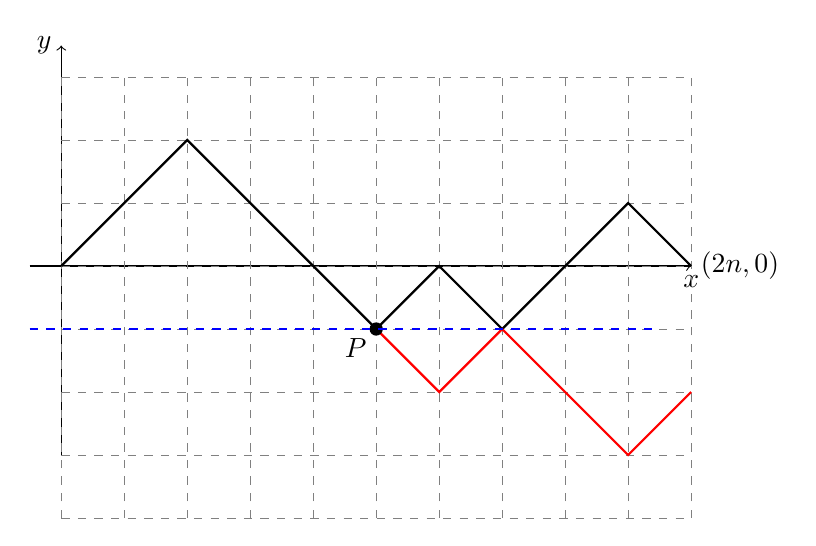
\begin{tikzpicture}[scale=0.8]
    % Axes
    \draw[->] (-0.5,0) -- (10,0) node[below] {\( x \)};
    \draw[->] (0,-3) -- (0,3.5) node[left] {\( y \)};

    % Grille
    \draw[help lines, dashed] (0,-4) grid (10,3);

    % Chemin initial (en noir)
    \draw[thick] (0,0) -- (1,1) -- (2,2) -- (3,1) -- (4,0) -- (5,-1) -- (6,0) -- (7,-1) -- (8,0) --
    (9,1) -- (10,0);

    % Chemin réfléchi (en rouge)
    \draw[thick, red] (5,-1) -- (6,-2) -- (7,-1) -- (8,-2) -- (9,-3) -- (10,-2);

    % Point de réflexion
    \fill[black] (5,-1) circle (3pt) node[below left] {\( P \)};

    % Axe de réflexion
    \draw[dashed, blue] (-0.5,-1) -- (9.5,-1);

    % Légende
    %\node[right, red] at (9,-1) {Réflexion du chemin};
    \node[right, black] at (10,0) {\( (2n,0) \)};
    %\node[right, blue] at (9,-1) {Axe \( y=-1 \)};
\end{tikzpicture}
